\documentclass[a4paper, 12pt]{article}
\usepackage{mhchem}
\usepackage{xcolor}
\usepackage{tikz}
\usepackage{chemfig}
\usepackage[
  left=3cm,
  right=2cm,
  top=2cm,
  bottom=2cm,
]{geometry}

\begin{document}
\section{Metalle mit Ingo}
\subsection{Eigenschaften metallischer Elemente}
Physikalische Eigenschaften
\begin{itemize}
    \item Leitfähigkeit
    \begin{itemize}
        \item elektrischen
        \item thermische
    \end{itemize}
    \item Metallischer Glanz
    \item Duktilität (Formbarkeit)
    \item Nicht Lichtdurchlässig
\end{itemize}
Chemische Eigenschaften
\begin{itemize}
    \item niedrige Elektronegativität
    \item bildet bevorzugt Kationen
    \item Meist basische Hydroxide!?
    \begin{itemize}
        \item niedrige Oxidationsstufe: JA \\Beispiel: \ce{Cr(OH)2 + H2O -> Cr^{2+} + 2OH- + H2O}
        \item hohe Oxidationsstufe: NEIN \\Beispiel: \ce{Cr(OH)6} (gibt's nicht) wird zu \ce{CrO2(OH)2} $->$\ce{H2CrO4}\\ \ce{H2CrO4 + 2H2O -> CrO4^{2-} + 2H3O+}
    \end{itemize}
\end{itemize}
\subsection{Elektrisches Verhalten}
\subsubsection{Betrachtung des spezifischen Widerstands}
\begin{itemize}
    \item Metalle: $10^{-4}$ bis $10^{-6} \Omega\cdot$ cm$^{-1}$
    \item Halbleiter: $10^{1}$ bis $10^{4} \Omega\cdot$ cm$^{-1}$
    \item Isolator: $> 10^{10} \Omega\cdot$ cm$^{-1}$
\end{itemize}
\subsubsection{Betrachtung der thermischen Verhaltens der Leitfähigkeit}
Siehe Folie
\subsection{Definition des metallischen Zustands}
Phänomenologisch: schwierig, da makroskopische Eigenschaften wie Glanz, Duktilität verändert werden können.\\
Temperaturabhängigkeit der elektrischen Leitfähigkeit: schwierig, da andere Stoffklassen ähnliche Eigenschaften aufweisen.
\subsection{Die chemische Bindung in Metallen}
\subsubsection{Ketelaar-Diagramm}
Man stelle sich ein Dreieck vor mit den Eckenbeschriftungen ionische Bindung \ce{NaCl}, kovalente Bindung \ce{Cl2} und metallisch \ce{Na}
\subsubsection{Das Elektronengasmodell}
\begin{itemize}
    \item Die Metallatome geben eine gewisse Zahl an Valenzelektronen ab, es verbleiben positiv geladene Atomrümpfe
    \item Die Elektronen sind zwischen den Atomrümpfen frei beweglich, ähnlich eines Gases $->$ Elektronengas \textcolor{red}{(versagt bei der Beschreibung der Wärmekapazität von Metallen)}
\end{itemize}
\subsubsection{Das Bändermodell}
\begin{itemize}
    \item Elektronen können nur bestimmte Energien aufweisen\\$->$ Orbitale (hier Atomorbitale)
    \item Beim Übergang von Ein- zu Mehratomsystemen\\$->$ Übergang von Atom- zu Molekülorbitalen
\end{itemize}
\ce{Li3}: $+\hspace*{0.25cm}+\hspace*{0.25cm}+\hspace*{0.25cm} = \sigma_b$\\
\hspace*{0.85cm}$+\hspace*{0.25cm}-\hspace*{0.25cm}+\hspace*{0.25cm} = \sigma_{ab}$\\
\hspace*{0.85cm}$+\hspace*{0.45cm}|\hspace*{0.45cm}+\hspace*{0.25cm} = \sigma_{nb}$
\begin{itemize}
    \item Beim Übergang von Mehr- zu Vielatomsystemen\\$->$ Übergang von Molekülorbital zu (Orbital-) Bändern\\$->$ Valenzband: mit Valenzelektronen besetzt, höchster besetzte Zustand: HOMO\\$->$ Leitungsband: frei, niedrigste unbesetzte Zustand: LUMO
\end{itemize}
Fermikante = Ort zwischen Besetzt und Unbesetzt\\
\subsection{Strukturen der Metalle}
Übersicht:
\begin{itemize}
    \item kubisch-innenzentriert
    \item hexagonal dichteste Packung
    \item kubisch dichteste Packung
    \item eigener Strukturtyp
    \item unbekannt
\end{itemize}
\subsubsection{Die kubisch-innenzentrierte Kugelpackung}
\textbf{(bcc = body-centered cubis), W(olfram)-Typ}
\\
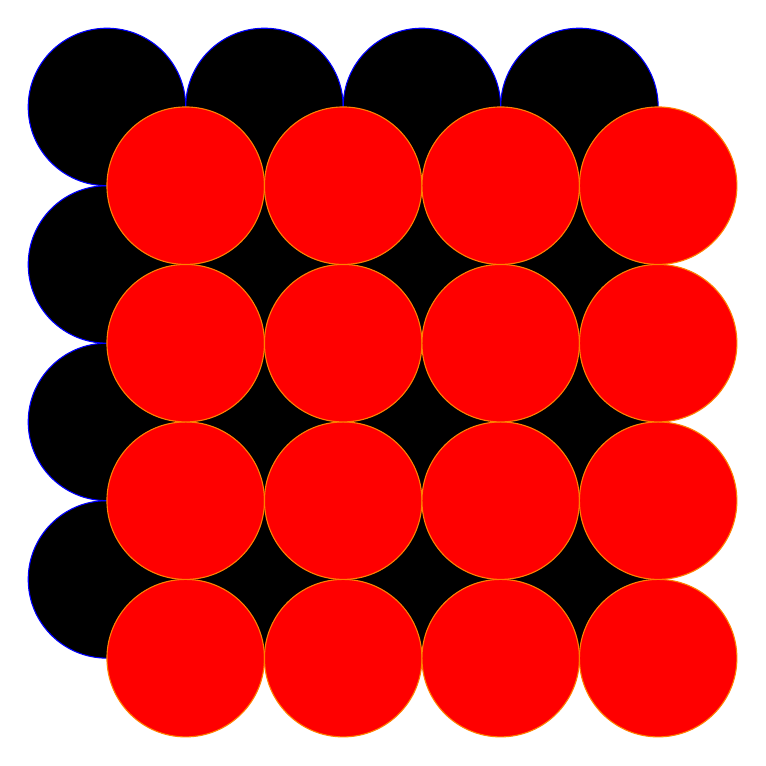
\begin{tikzpicture}
    \draw[color=blue,fill=black] (0,0) circle (1cm);
    \draw[color=blue,fill=black] (2,0) circle (1cm);
    \draw[color=blue,fill=black] (4,0) circle (1cm);
    \draw[color=blue,fill=black] (6,0) circle (1cm);
    \draw[color=blue,fill=black] (0,2) circle (1cm);
    \draw[color=blue,fill=black] (2,2) circle (1cm);
    \draw[color=blue,fill=black] (4,2) circle (1cm);
    \draw[color=blue,fill=black] (6,2) circle (1cm);
    \draw[color=blue,fill=black] (0,4) circle (1cm);
    \draw[color=blue,fill=black] (2,4) circle (1cm);
    \draw[color=blue,fill=black] (4,4) circle (1cm);
    \draw[color=blue,fill=black] (6,4) circle (1cm);
    \draw[color=blue,fill=black] (0,6) circle (1cm);
    \draw[color=blue,fill=black] (2,6) circle (1cm);
    \draw[color=blue,fill=black] (4,6) circle (1cm);
    \draw[color=blue,fill=black] (6,6) circle (1cm);
    \draw[color=orange,fill=red] (1,-1) circle (1cm);
    \draw[color=orange,fill=red] (3,-1) circle (1cm);
    \draw[color=orange,fill=red] (5,-1) circle (1cm);
    \draw[color=orange,fill=red] (7,-1) circle (1cm);
    \draw[color=orange,fill=red] (1,1) circle (1cm);
    \draw[color=orange,fill=red] (3,1) circle (1cm);
    \draw[color=orange,fill=red] (5,1) circle (1cm);
    \draw[color=orange,fill=red] (7,1) circle (1cm);
    \draw[color=orange,fill=red] (1,3) circle (1cm);
    \draw[color=orange,fill=red] (3,3) circle (1cm);
    \draw[color=orange,fill=red] (5,3) circle (1cm);
    \draw[color=orange,fill=red] (7,3) circle (1cm);
    \draw[color=orange,fill=red] (1,5) circle (1cm);
    \draw[color=orange,fill=red] (3,5) circle (1cm);
    \draw[color=orange,fill=red] (5,5) circle (1cm);
    \draw[color=orange,fill=red] (7,5) circle (1cm);
\end{tikzpicture}\\
\underline{C}oordination\underline{N}umber = 8 + 6\\
Koordinationspolyeder = Rhombododecaeder\\
Raumerfüllung = 68\%\\
Siehe Folie für näheres.
\newpage
\subsubsection{Die dichtesten Packungen}
\textbf{Hexagonal-dichteste Kugelpackung\\(hcp = hexagonal close packed), M(a)g(nesium)-Typ}
\\\\
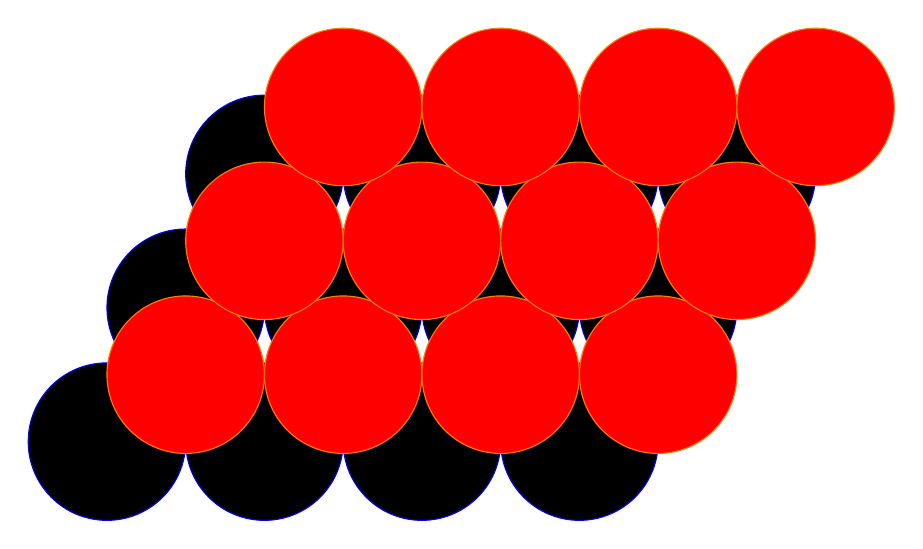
\begin{tikzpicture}
    \draw[color=blue,fill=black] (0,0) circle (1cm);
    \draw[color=blue,fill=black] (2,0) circle (1cm);
    \draw[color=blue,fill=black] (4,0) circle (1cm);
    \draw[color=blue,fill=black] (6,0) circle (1cm);
    \draw[color=blue,fill=black] (1,1.7) circle (1cm);
    \draw[color=blue,fill=black] (3,1.7) circle (1cm);
    \draw[color=blue,fill=black] (5,1.7) circle (1cm);
    \draw[color=blue,fill=black] (7,1.7) circle (1cm);
    \draw[color=blue,fill=black] (2,3.4) circle (1cm);
    \draw[color=blue,fill=black] (4,3.4) circle (1cm);
    \draw[color=blue,fill=black] (6,3.4) circle (1cm);
    \draw[color=blue,fill=black] (8,3.4) circle (1cm);
    \draw[color=orange,fill=red] (1,0.85) circle (1cm);
    \draw[color=orange,fill=red] (3,0.85) circle (1cm);
    \draw[color=orange,fill=red] (5,0.85) circle (1cm);
    \draw[color=orange,fill=red] (7,0.85) circle (1cm);
    \draw[color=orange,fill=red] (2,2.55) circle (1cm);
    \draw[color=orange,fill=red] (4,2.55) circle (1cm);
    \draw[color=orange,fill=red] (6,2.55) circle (1cm);
    \draw[color=orange,fill=red] (8,2.55) circle (1cm);
    \draw[color=orange,fill=red] (3,4.25) circle (1cm);
    \draw[color=orange,fill=red] (5,4.25) circle (1cm);
    \draw[color=orange,fill=red] (7,4.25) circle (1cm);
    \draw[color=orange,fill=red] (9,4.25) circle (1cm);
\end{tikzpicture}\\
CN=12\\
Koordinationspolyeder = Antikuboktaeder\\
Raumerfüllung = 74\%\\\\
\textbf{Kubisch-dichteste Kugelpackung\\(ccp=cubic close packed), Cu(pfer)-Typ}
\\\\
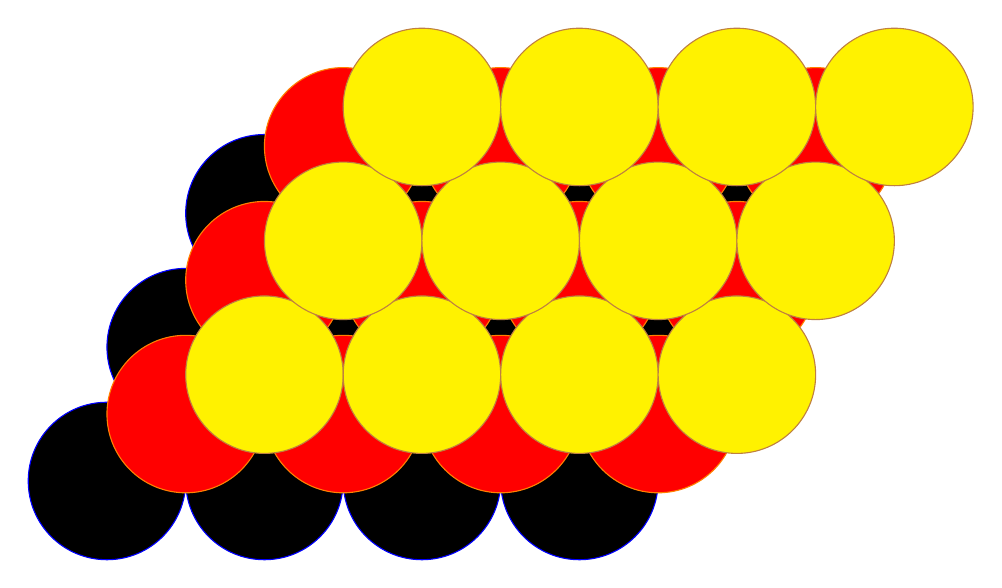
\begin{tikzpicture}
    \draw[color=blue,fill=black] (0,0) circle (1cm);
    \draw[color=blue,fill=black] (2,0) circle (1cm);
    \draw[color=blue,fill=black] (4,0) circle (1cm);
    \draw[color=blue,fill=black] (6,0) circle (1cm);
    \draw[color=blue,fill=black] (1,1.7) circle (1cm);
    \draw[color=blue,fill=black] (3,1.7) circle (1cm);
    \draw[color=blue,fill=black] (5,1.7) circle (1cm);
    \draw[color=blue,fill=black] (7,1.7) circle (1cm);
    \draw[color=blue,fill=black] (2,3.4) circle (1cm);
    \draw[color=blue,fill=black] (4,3.4) circle (1cm);
    \draw[color=blue,fill=black] (6,3.4) circle (1cm);
    \draw[color=blue,fill=black] (8,3.4) circle (1cm);
    \draw[color=orange,fill=red] (1,0.85) circle (1cm);
    \draw[color=orange,fill=red] (3,0.85) circle (1cm);
    \draw[color=orange,fill=red] (5,0.85) circle (1cm);
    \draw[color=orange,fill=red] (7,0.85) circle (1cm);
    \draw[color=orange,fill=red] (2,2.55) circle (1cm);
    \draw[color=orange,fill=red] (4,2.55) circle (1cm);
    \draw[color=orange,fill=red] (6,2.55) circle (1cm);
    \draw[color=orange,fill=red] (8,2.55) circle (1cm);
    \draw[color=orange,fill=red] (3,4.25) circle (1cm);
    \draw[color=orange,fill=red] (5,4.25) circle (1cm);
    \draw[color=orange,fill=red] (7,4.25) circle (1cm);
    \draw[color=orange,fill=red] (9,4.25) circle (1cm);
    \draw[color=brown,fill=yellow] (2,1.35) circle (1cm);
    \draw[color=brown,fill=yellow] (4,1.35) circle (1cm);
    \draw[color=brown,fill=yellow] (6,1.35) circle (1cm);
    \draw[color=brown,fill=yellow] (8,1.35) circle (1cm);
    \draw[color=brown,fill=yellow] (3,3.05) circle (1cm);
    \draw[color=brown,fill=yellow] (5,3.05) circle (1cm);
    \draw[color=brown,fill=yellow] (7,3.05) circle (1cm);
    \draw[color=brown,fill=yellow] (9,3.05) circle (1cm);
    \draw[color=brown,fill=yellow] (4,4.75) circle (1cm);
    \draw[color=brown,fill=yellow] (6,4.75) circle (1cm);
    \draw[color=brown,fill=yellow] (8,4.75) circle (1cm);
    \draw[color=brown,fill=yellow] (10,4.75) circle (1cm);
\end{tikzpicture}\\
CN = 12\\
Koorinationspolyeder = Kuboktaeder\\\\
\textbf{Varianten der dichtesten Kugelpackungen}\\
hc-Typ\\
hhc-Typ\\
Kommen vor und nach einer Schicht dieselbe Schicht, so ist diese hexagonal umgeben. (Kurz: h)\\
Sind die Schichten vor und nach der betrachteten Schicht nicht gleich, so ist die betrachtete Schicht kubisch umgeben. (Kurz: c)\\\\
Siehe Folie.\\\\
\textbf{Variation der Kristallstruktur der Metalle.\\(Abhängig von Druck und Temperatur)}\\\\
\ce{Fe}: \ce{$\alpha \left(\mathrm{bcc}\right)$ -> $\gamma \left(\mathrm{ccp}\right)$ -> $\delta \left(\mathrm{bcc}\right)$}\\
Erster Schritt bei ca. 900$^\circ$, zweiter schritt bei ca. 1400$^\circ$\\\\
\ce{Na}: bcc \ce{->} ccp \ce{-> -> ->} transparente Modifikation, kein Metall mehr\\
Dabei läuft der erste Schritt bei 656 Pa ab und der letzte bei $>$ 100 GPa
\subsubsection{Aufgefüllte dichteste Packungen}
\begin{itemize}
    \item Oktaederlücken\\hcp-Abfolge: A c B (A,B = Schichten, c = Lücken)\\$N(\mathrm{Oktaederl\text{ü}cken})=N(\mathrm{Packungsteilchen})$\\
            ccp Abfolge: A c B a C b A (A,B,C = Schichten, a,b,c = Lücken)
    \item Tetraederlücken\\hcp:Abfolge: A $\beta$ $\alpha$ B $\alpha$ $\beta$ A $\beta$ (A,B = Schichten, $\alpha, \beta$ = Lücken)\\$N(\mathrm{Tetraederl\text{ü}cken})=2N(\mathrm{Packungsteilchen})$\\Tetraederlücken\\
            ccp:Abfolge: A $\beta$ c $\alpha$ B $\gamma$ a $\beta$ C $\alpha$ b $\gamma$ A (A,B,C = Schichten, $\alpha, \beta, \gamma$ = Tetraederlücken, a, b, c = Oktaederlücken)
\end{itemize}

\subsection{Die Elemente der ersten und elften Periode (-\ce{H}$\&$\ce{Rg})}
\begin{itemize}
    \item[1. Gruppe] Alkalimetalle
    \item[11. Gruppe] Münzmetalle 
\end{itemize}
\subsubsection{Vorkommen}
\begin{itemize}
    \item[Alkalimetalle]:
    \begin{itemize}
        \item kationisch in salzartifen Verbindungen \ce{NaCl} - Halit, \ce{KCl} -Sylvin
        \item kationisch eingelagert in Alumosilicaten (\ce{LiAlSi2O6})
    \end{itemize}
    \item[Münzmetalle]:
    \begin{itemize}
        \item[Kupfer:] hauptsächlich sulfidisch: \ce{Cu2S}, \ce{CuFeS2}, $\dots$\\auch: gediegen (elementar)
        \item[Silber:] hauptsächlich gediegen\\auch: sulfidisch
        \item[Gold:] hauptsächlich gediegen\\selten: Goldtelluride  
    \end{itemize}
\end{itemize}
\subsubsection{Herstellung}
\begin{itemize}
    \item[Alkalimetalle]:
    \begin{itemize}
        \item[\ce{Li} und  \ce{Na}:] Schmelzflusselektrolyse aus Salz(-mischungen)
        \item[\ce{K}:] Reduktion mit metallischem \ce{Na}
        \item[\ce{Rb} und \ce{Cs}:] Reduktion mit metallischem \ce{Ca} und anschließender Destillation
    \end{itemize}
    \item[Münzmetalle]:
    \begin{itemize}
        \item[\ce{Cu}:] Rösten der sulfideischen Kupfererze\\Rösten: \ce{6CuFeS2 + 13O2 -> 3Cu2S + 2Fe3O4 + 9SO2}\\Schlacke: \ce{2Fe3O4 + 2CO + 3 SiO2 -> 3Fe2SiO4 + 2 CO2}\\$\rightarrow$(Abtrennug des Eisenanteils)\\\begin{center}\ce{2Cu2S + 3O2 -> 2 Cu2O + 2SO2}\end{center}\begin{tabular}{c | c}Röstreaktion & Röstreduktion\\\ce{2Cu2O + Cu2S -> 6Cu + SO2$\uparrow$}&\ce{Cu2O + CO -> 2Cu + CO2$\uparrow$}\end{tabular}\\Reinigung des Rohkupfers durch elektrolytische Kupferaffinition
        \item[\ce{Ag} und \ce{Au}:] Reinigung der gediegenen Metalle
        \begin{itemize}
            \item Recycling aus Anodenschlamm (Reinigung des Rohkupfers)
            \item Amalgamierung vom Gold, Goldwäsche
            \item Cyanidlaugerei\\\ce{Ag2S + 4NaCN -> 2Na[Ag(CN)2] + Na2S}\\\ce{2Ag + H2O + 1/2O2 + 4NaCN -> 2Na[Ag(CN)2] + 2 NaOH}\\\\\ce{Ag^+ + 2CN^- -> [Ag(CN)2]^-} $K_K \approx 10^{21}\mathrm{\frac{mol^2}{l^2}}$\\$K_K=\frac{\ce{[[Ag(CN)2]^-]}}{[\ce{Ag^+}]\cdot\ce{[CN^-]^2}} \rightarrow \ce{[Ag^+]} = \frac{\ce{[[Ag(CN)2]^-]}}{K_K\cdot\ce{[CN^-]^2}}$\\$E=E^o_{(\ce{Ag}/\ce{Ag^+})}+\frac{RT}{zF}\ln([\ce{Ag^+}])$\\\\Rückgewinnung des Silbers\\\ce{2Na[Ag(CN)2] + Zn -> 2Ag + Na2[Zn(CN)4]}
        \end{itemize}
    \end{itemize}
\end{itemize}
\subsubsection{Verbindungen}
\begin{itemize}
    \item[Halogenide]:
    \begin{itemize}
        \item Alkalimetallhalogenide: \ce{A} = \ce{Li} bis \ce{Cs} $\rightarrow$ \ce{AX} $\leftarrow$ \ce{X} = \ce{F} bis \ce{I}
        \item[] \ce{NaCl}-Struktur: ccp mit allen Oktaederlücken gefüllt
        \item[] \ce{CsCl}-Struktur: kubisch-primitiver Aufbau der Packungsteilchen, Lückensitzer im Zentrum des Würfels 
    \end{itemize}
    \item[Münzmetalle]:
    \begin{itemize}
        \item[] Cu(I)-Halogenide vom \chemfig{Cl-I}
        \item[] Cu(II)-Halogenide $\rightarrow$ schwache Oxidationsmittel
        \item[] \ce{CuCl2 + Cu -> CuCl} $\ce{->[\mathrm{mehr} \ce{Cl^-}] CuCl_{2/3/4}^{1/2/3 -}}$
        \item[] \ce{CuCl2 + Fe^{2+} -> CuCl + Fe^{3+} + Cl^-}
        \item[] \ce{CuI2 -> CuI + 1/2I2}
        \item[] \ce{Cu^{2+} + 2 CN^- -> CuCN + 1/2 (CN)2}
        \item[] Oxidation organischer Verbindungen $\rightarrow$ Fehling-Probe
        \item[] \ce{Ag^+} + Halogenide $\rightarrow$ \ce{AgF}, \ce{AgCl}, \ce{AgBr}, \ce{AgI} 
    \end{itemize}
\end{itemize}
\subsubsection{Sauerstoff-Verbindungen}
\begin{itemize}
    \item[] \ce{4Li + O2 -> 2Li2O}
    \item[] \ce{6Li + N2 -> 2Li3N}
    \item[] \ce{2Na + O2 -> 2NaO ->[{besser}] Na2O2} - natriumperoxid (\ce{O2^{-2}})
    \item[] \ce{A + O2 -> AO2} mit \ce{A} = \ce{K}, \ce{Rb}, \ce{Cs} \\ Der Name des \ce{AO2} lautet: "Alkalimetallsuperoxid" $\rightarrow$ \ce{O2^-}
    \item[] Umsetzung mit mehr \ce{O2}:
    \item[] \ce{A4O6} $\rightarrow$ 1$\times$ \ce{O2^{-2}} + 2 $\times$ \ce{O2^-}
    \item[] Umsetzung mit Metallüberschuss $\rightarrow$ Alkalimetallsuboxide
\end{itemize}
Münzmetalle
\begin{itemize}
    \item[] \ce{Cu2O} rot; \ce{CuO} schwarz
    \item[] \ce{Ag2O}, \ce{AgO} aber \ce{Ag^I Ag^{II} O2}
    \item[] \ce{AuO} -"- \ce{Au2O3}
\end{itemize}

\subsubsection{Hydroxide}
\begin{itemize}
    \item Alkalimetallhydroxide
    \begin{itemize}
        \item stark basisch
        \item ziehen \ce{CO2} aus der Luft
    \end{itemize}
    \item Herstellung durch Elektrolyse aus NaCl-Lösung
    \begin{itemize}
        \item Chloralkalielektrolyse
        \item[] \ce{2NaCl + 2H2O ->[{Strom}] 2Na^+ + 2OH^- + Cl2 + H2}
        \item[Probleme:] \ce{Cl2} disproportioniert in Lauge\\\ce{H2 + Cl2 ->} Chlorknallgas 
    \end{itemize}
    \item Münzmetallhydroxide
    \begin{itemize}
        \item \ce{Cu(OH)2}
        \item \ce{Au(OH)3}
        \item[] \ce{2A + 2H2O -> A^+ + OH^- + H2}
    \end{itemize}
\end{itemize}

\subsubsection{Alkalimetall-Elektrode und Alkalide}
\begin{center}
    \ce{A -> A^+ + e^-}\\
    $\hookrightarrow$ \ce{+ 3-4 NH3 -> [e(NH3)_{3-4}]^-}
\end{center}
auch möglich:\\
\ce{A} + $\begin{array}{c}Kronenether\\ Cryptant\end{array}$ \ce{->} [A(Kronenether)]$^+$ + e$^-$ \ce{->[{+A}]} [A(Kronenether)]$^+$ + A$^-$
\subsubsection{Stickstoffverbindungen}
\begin{itemize}
    \item[$\rightarrow$] Nitride \ce{N^{3-}}
    \item[$\rightarrow$] Imide \ce{NH^{2-}} (vgl. \ce{O^{2-}})
    \item[$\rightarrow$] Amide \ce{NH2^-} (vgl. \ce{OH^- H^-})
    \item[$\rightarrow$] Ammoniak \ce{NH3} (vgl. \ce{H2O HF})
    \item[$\rightarrow$] Ammonium \ce{NH4^+} (vgl. \ce{H3O^+ H2F^+} \textcolor{gray}{$\rightarrow$ \ce{CH4}})
    \item[$\rightarrow$] Azide \ce{N3^-} (isoelektronisch zu \ce{N2O CO2 NO2^+})
\end{itemize}

\subsection{Oxidationsstufen der Münzmetalle}
\subsubsection{Allgemeines}
$\hookrightarrow$ Siehe Folie\\
Wiederholung der Kristallfeldtheorie\\
$\hookrightarrow$ Siehe Folie\\

\subsubsection{Verbindungen von \ce{Cu} und \ce{Ag} in hohen Oxidationsstufen}
\ce{CuF3, K3[CuF6], 4Ba2Cu3O_{7-x}} (Supraleiter)\\
\ce{K[AgF4], Cs2[AgF4]}

\subsection{Die Chemie der Golds}
\subsubsection{Relativistische Effekte}
Kontraktion von 6s und 6p; Expansion von 5d
\begin{itemize}
    \item $r$(Au) $\approx r$(Ag) $\rightarrow$ höhere dichte
    \item höhere Elektronenaffinität $\rightarrow$ \ce{Au^-} aber kein \ce{Ag^-}
    \item aurophile Wechselwirkungen $\rightarrow$ \chemfig{Au-Au}-Bindungen in der Gasphase
    \item Farbigkeit $\rightarrow$ elektronische Übergäng eim sichtbaren Bereich
\end{itemize}

\subsubsection{Goldverbindungen}
Oxidation von Gold durch Königswasser
\begin{itemize}
    \item[] \ce{HNO3 + 3HCl -> NO4 + 2H2O + 2Cl$\cdot$}\\\ce{Cl$\cdot$} ist das naszierende Chlor
    \item[] \ce{Au + 3Cl$\cdot$ + Cl^- -> [AuCl4]^-} \textcolor{gray}{(Tetrachloridoaurat)}
    \item \ce{Au^{2+}} $\mathrm{5d^9}$-System $\rightarrow$ \ce{Au2^{4+}}
\end{itemize}
\end{document}